\documentclass[preprint,12pt]{elsarticle}

\journal{Information Sciences}
\biboptions{numbers,sort&compress}

\usepackage{amsmath,amssymb,amsfonts}
\usepackage{amsthm}
\usepackage{graphicx}
\usepackage{booktabs}
\usepackage{xcolor}
\usepackage{url}
\usepackage{lineno}
\usepackage[hidelinks]{hyperref}

\graphicspath{{figures/}}

\newcommand{\system}{\textsc{TrustRoute}}
\newcommand{\rel}{\mathrm{rel}}
\newcommand{\cost}{\mathrm{cost}}
\newcommand{\trust}{\mathrm{trust}}

\newtheorem{proposition}{Proposition}
\newtheorem{definition}{Definition}
\newtheorem{remark}{Remark}

\begin{document}

\begin{frontmatter}

\title{Trust as a First-Class Routing Objective: Provenance-Robust Resource
Selection for AI-Native Data Systems}

\author[scch]{Jorge Martinez-Gil\corref{cor1}}
\ead{jorge.martinez-gil@scch.at}
\cortext[cor1]{Corresponding author.}
\affiliation[scch]{
  organization={Software Competence Center Hagenberg GmbH (SCCH)},
  city={Hagenberg im Muehlkreis},
  postcode={4232},
  country={Austria}
}

\begin{abstract}
AI-native data systems answer queries by routing among heterogeneous sources:
relational tables, vector indexes, retrieval services, model-backed tools, and
third-party or machine-generated stores. Classical resource selection ranks
sources by content, but content alone cannot distinguish a curated source from an
untrusted duplicate whose text is lexically identical and whose answers may be
stale, poisoned, or unverifiable. We formalize provenance-robust resource
selection and prove a content-only impossibility bound: with $m$
content-identical impostors, no content-only router can choose the genuine source
with probability above $1/(m+1)$ inside the equivalence class. We instantiate
trust as a first-class routing objective in \system, which multiplies a standard
CORI relevance signal by an online beta--binomial trust estimate and routes by
expected utility under a cost budget. On a reproducible federation of six real
information-retrieval collections (23{,}709 documents; 776 judged queries),
\system{} remains competitive on a clean federation and is markedly more robust
under contamination. With eight evil-twin sources, CORI's routing accuracy drops
from $0.893$ to $0.431$, whereas \system{} retains $0.787$, preserving $96\%$ of
clean routing accuracy and $96\%$ of clean nDCG@10. At six twins, \system{}
improves nDCG@10 over CORI by $+0.193$ and over ReDDE by $+0.217$, with
Holm-corrected paired Wilcoxon tests giving $p\le 4.9\times10^{-59}$ and large
effects. Additional experiments show that the posterior recovers graded
reliability, tracks non-stationary drift, and is stable across a $4\times3$
hyper-parameter grid.
\end{abstract}

\begin{keyword}
resource selection \sep federated search \sep query routing \sep data provenance
\sep trust calibration \sep retrieval-augmented generation \sep AI-native systems
\end{keyword}

\end{frontmatter}

\linenumbers

\section{Introduction}

Modern data systems are no longer closed catalogs of trusted tables. A single
analytical or conversational query may be served by a vector index, a lexical
search service, a relational store, a model-backed tool, an external knowledge
API, or a passage generated on the fly~\cite{lewis2020rag,gao2023rag,
ooi2024neurdb,zhou2025llmdata}. We call such systems \emph{AI-native}: the unit of execution is
no longer a stable operator over curated data but a \emph{source} whose
reliability, freshness, cost, and---critically---\emph{trustworthiness} vary
widely and drift over time.

The component that decides \emph{which source(s) to query} is a
\emph{resource-selection} or \emph{query-routing} layer, studied for decades in
federated and distributed information retrieval~\cite{callan1995cori,
si2003redde,callan2000distributed,shokouhi2011federated}. Classical methods rank
candidate sources by how well their \emph{content} statistics match the query.
This works well when every source is trustworthy. It fails---silently and
catastrophically---when some sources are not.

\subsection{Why this is now a first-order concern}
Provenance-blindness has always been latent in federated retrieval, but three
concurrent shifts in how data systems are built have turned it from a corner case
into a first-order design problem.

\emph{Open data planes and agent tool servers.} Retrieval is increasingly
brokered across many third-party endpoints registered dynamically rather than
curated once. Protocols such as the Model Context Protocol~\cite{anthropic2024mcp}
let an agent discover and call external tool and data servers at run time, and
``data management for AI'' systems treat such heterogeneous sources as
first-class~\cite{ooi2024neurdb,zhou2025llmdata}. The router now stands in front
of endpoints that no one has vetted end-to-end.

\emph{Adversarial contamination.} Retrieval corpora are demonstrably attackable.
Corpus-poisoning attacks craft a handful of adversarial passages that are
retrieved for many queries~\cite{zhong2023corpus}, and knowledge-corruption
attacks such as PoisonedRAG show that injecting a few malicious documents can
flip the answers of a retrieval-augmented generator~\cite{zou2025poisonedrag}. A
poisoned or hallucinated store can be \emph{lexically indistinguishable} from a
genuine one while returning unverifiable content.

\emph{Routing-as-control.} As pipelines add learned and agentic
routers~\cite{singh2025agentic,zhang2025ragrouter}, the routing decision---not
just the ranking inside a single index---determines answer quality. If routing is
optimized for relevance alone, it inherits exactly the blind spot that
contamination exploits.

\paragraph*{The provenance-blindness problem}
Consider a federation that contains, alongside a curated source, an
\emph{untrustworthy duplicate} of it: a scraped copy hosted by an unverified
third party, a stale replica, a poisoned store, or a retrieval store populated by
a hallucinating model. Such a source is, by construction, \emph{lexically
indistinguishable} from the genuine one. Any selector that ranks sources by
content statistics must treat the two identically and will route to the impostor
roughly half the time. Because the impostor's answers cannot be trusted---they
may be tampered, outdated, or fabricated---this halves end-to-end answer quality
even though the \emph{retrieval} machinery is working perfectly. Content is simply
the wrong signal: the distinguishing property is
\emph{provenance}~\cite{buneman2001why}, not text. No amount of better term
matching can close a gap that lives in a dimension term matching cannot see.

\paragraph*{Trust as a first-class objective}
We argue that an AI-native router must optimize \emph{trust} as a first-class
objective, on equal footing with relevance and cost. Crucially, trust cannot be
read off a source's content; it must be \emph{learned from observed outcomes}---
did routing to this source actually satisfy the information need? We instantiate
this idea in \system, a router that (i) computes a standard content-relevance
signal, (ii) maintains a per-source \emph{calibrated} trust estimate as a
beta--binomial posterior with an optimistic prior and a lower confidence bound,
updated online from routing outcomes, and (iii) routes by \emph{expected utility}
$=\rel\times\trust$ under a cost budget. At cold start trust is uniform and
\system{} reduces \emph{exactly} to its content baseline; as evidence accrues,
unreliable sources are multiplicatively suppressed. The design is deliberately
minimal: one beta--binomial pair per source, an $O(1)$ update, and no change to
the underlying retriever.

\paragraph*{Headline result}
On a fully reproducible federation of six real IR collections, the gap is stark
(Fig.~\ref{fig:robust}). When the federation is diluted with eight evil-twin
sources---so that impostors outnumber genuine sources ($8$ of $14$)---content-based
routing accuracy collapses to $0.431$ (CORI) and $0.396$ (ReDDE), roughly half of
their clean values. \system{} holds at $0.787$, essentially unchanged from its
clean $0.822$. Stated as \emph{robustness retention}---the fraction of clean
accuracy preserved under maximal contamination---\system{} keeps $96\%$ while
content baselines keep $48$--$50\%$ (Table~\ref{tab:sweep}). The same pattern
holds for end-to-end nDCG@10 and MAP, is significant after multiplicity
correction, and comes at an average query cost below both content baselines at
\system's single-source operating point.

\paragraph*{Contributions}
\begin{itemize}
\item We formalize \emph{provenance-robust resource selection}, give an
expected-utility objective that places trust on equal footing with relevance and
cost, and show, on real data, that content-based selection is structurally blind
to provenance (Sections~\ref{sec:problem},~\ref{sec:threat}).
\item We prove a \emph{content-only impossibility bound}: any router that observes
only content can place a genuine source first with probability at most $1/(m{+}1)$
in a class with $m$ content-identical impostors, no matter how good the term
matcher (Proposition~\ref{prop:bound}).
\item We present \system, which combines a content-relevance signal with an
online-calibrated beta--binomial trust estimate and routes by expected utility
under a cost budget, reducing to its content baseline at cold start, with an
$O(1)$ trust update and a complexity analysis (Section~\ref{sec:method}).
\item We assemble a fully reproducible federated testbed from six real,
heterogeneous IR collections and evaluate against established baselines (CORI,
ReDDE) with statistical rigor: query-clustered paired Wilcoxon tests,
family-wise Holm--Bonferroni correction, query-bootstrap confidence intervals,
and matched-pairs rank-biserial effect sizes over three seeds
(Section~\ref{sec:setup}).
\item We characterize robustness as a \emph{contamination sweep} ($0$ to $8$
twins) rather than a single point, introduce a retention metric that summarizes
graceful degradation, and report a budget analysis showing where the trust
signal helps and where it does not (Section~\ref{sec:results}).
\item We \emph{generalize the threat model} beyond exact twins
(Section~\ref{sec:extended}): graded/stochastic poisoning, where the posterior
recovers true reliability; non-stationary drift, where the online estimator
re-calibrates; and a hyper-parameter sweep that maps the method's robust
operating region and its one honestly reported degenerate corner.
\item We report negative and null results candidly, including the modest cost of
the mechanism on clean data and the boundary at which content statistics become
informative again.
\end{itemize}

\paragraph*{Organization}
Section~\ref{sec:related} surveys related work. Section~\ref{sec:problem}
formalizes provenance-robust resource selection and Section~\ref{sec:threat} the
untrusted-source threat model, including the impossibility bound.
Section~\ref{sec:method} presents \system. Sections~\ref{sec:setup}
and~\ref{sec:results} give the setup and the core results (RQ1--RQ7),
Section~\ref{sec:extended} the generalized threat model (RQ8--RQ10), and
Sections~\ref{sec:discussion}--\ref{sec:conclusion} discuss limitations and
conclude.

\section{Related Work}\label{sec:related}

\paragraph*{Resource selection and federated search}
Resource selection ranks collections by their likely usefulness for a query.
CORI~\cite{callan1995cori} treats each collection as a ``big document'' and scores
it with an inference-network belief built from per-collection document and
collection frequencies. Sample-based methods such as ReDDE~\cite{si2003redde}
estimate the number of relevant documents in each collection by ranking a
centralized sample and scaling by collection size. Surveys
\cite{callan2000distributed,shokouhi2011federated} map the broader space. All of
these methods are \emph{content-based}: they are blind to whether a source's
documents can be trusted, which is precisely the failure mode we study. Our
contribution is orthogonal to the choice of content signal---we use CORI's, and
add a trust factor that any of these scorers could carry.

\paragraph*{Retrieval-augmented generation and learned routing}
RAG pipelines~\cite{lewis2020rag,gao2023rag} and learned re-rankers
\cite{nogueira2019passage} have renewed interest in choosing \emph{where} to
retrieve. A recent line of work makes the router itself learned or agentic:
agentic RAG systems plan multi-step retrieval and tool use~\cite{singh2025agentic},
and learned RAG routers select among retrievers or knowledge sources per
query~\cite{zhang2025ragrouter}. These systems optimize routing for relevance,
latency, or cost; the trustworthiness of the chosen source is typically assumed
rather than estimated. Our work supplies that missing objective and shows it is
necessary, not merely beneficial: on a contaminated federation, optimizing
relevance alone is provably insufficient because relevance cannot separate a twin
from its original (Proposition~\ref{prop:bound}). \system{} is complementary to a
learned router: its calibrated trust factor can be carried by any relevance
scorer, learned or hand-built.

\paragraph*{Adversarial contamination and corpus poisoning}
A growing body of work shows retrieval corpora are attackable. Corpus-poisoning
attacks craft adversarial passages that a dense retriever surfaces for a broad
set of queries~\cite{zhong2023corpus}; knowledge-corruption attacks such as
PoisonedRAG inject a small number of malicious documents to control a RAG
system's output~\cite{zou2025poisonedrag}. These defenses operate at the
\emph{document} level---detecting or filtering individual poisoned passages.
\system{} is a \emph{routing-layer} defense, complementary to document-level
ones: it asks not ``is this passage poisoned?'' but ``has this \emph{source}
historically satisfied information needs?'', and it suppresses a source whose
outcomes are unreliable regardless of why. The two layers compose: document
filters reduce the per-query poison rate, and the trust layer demotes sources
that remain unreliable in aggregate.

\paragraph*{Open data planes, tool servers, and data management for AI}
AI-native data management treats heterogeneous, dynamically registered sources as
first-class citizens~\cite{ooi2024neurdb,zhou2025llmdata}, and agent protocols such
as the Model Context Protocol~\cite{anthropic2024mcp} make run-time discovery of
external tool and data servers routine. This is exactly the setting in which a
source's provenance cannot be assumed: endpoints appear and disappear, mirrors
proliferate, and the router must decide whom to trust from behavior, not from a
static registry. We position provenance-robust routing as a primitive for this
emerging stack.

\paragraph*{Provenance, trust, and calibration}
Data provenance characterizes \emph{why} and \emph{where} data originates
\cite{buneman2001why}; we operationalize a downstream consequence---a source
whose provenance cannot be verified should not be trusted even when its content
matches. Our trust estimator is a beta--binomial posterior summarized by a lower
confidence bound~\cite{wilson1927interval,brown2001interval} under an optimistic
prior, connecting to optimism-under-uncertainty in bandits~\cite{auer2002finite}.
Unlike a bandit that seeks to maximize cumulative reward by exploration, our aim
is \emph{calibrated suppression}: we want the posterior to track each source's
true reliability so that routing degrades gracefully, which is why we summarize by
a conservative lower bound rather than an optimistic upper one. For evaluation we
follow best practice for comparing methods across many
queries~\cite{demsar2006statistical}: the Wilcoxon signed-rank
test~\cite{wilcoxon1945individual}, Holm correction~\cite{holm1979simple}, and
matched-pairs rank-biserial effect sizes~\cite{cliff1993delta}.

\section{Problem Formulation}\label{sec:problem}

\begin{definition}[Federation]
A \emph{federation} is a set of sources $\mathcal{C}=\{c_1,\dots,c_n\}$. Each
source $c_i$ holds a document collection $D_i$ and answers a query $q$ by
returning a ranked list $R_i(q)$ via a local retrieval model (here Okapi
BM25~\cite{robertson2009bm25}). Each source has a cost $\cost(c_i)$ and a latency
profile.
\end{definition}

A \emph{router} receives a query $q$ and a budget $b$ and must choose an ordered
subset $S(q)\subseteq\mathcal{C}$, $|S(q)|\le b$, to query; results from the
selected sources are merged into a single ranking $R_{S}(q)$. We measure
\emph{routing accuracy}~$R@k$ (is a source containing relevant documents selected
within the top $k$?), \emph{reciprocal rank} of the best source, and
\emph{end-to-end} retrieval quality (nDCG@10, MAP) of $R_{S}(q)$, each as a
function of the cost budget $b$.

\subsection{An expected-utility objective}
We make trust an explicit term in the routing objective rather than a
post-hoc filter. Let $\rel(c_i,q)\in[0,1]$ be a content-relevance score and let
$\trust(c_i)\in[0,1]$ be a reliability estimate---the probability that routing to
$c_i$ satisfies an information need. We define the \emph{expected utility} of
querying $c_i$ for $q$ as
\begin{equation}
u(c_i,q)\;\propto\;\rel(c_i,q)\cdot\trust(c_i)\;-\;\lambda\,\widehat{\cost}(c_i),
\label{eq:utility}
\end{equation}
and route to the budget-constrained subset maximizing $\sum_{c\in S}u(c,q)$. The
multiplicative coupling of relevance and trust is the crux: a highly relevant but
untrusted source has \emph{low} utility, so it is demoted exactly when content
scoring would promote it. Setting $\trust(c_i)\equiv 1$ recovers a classical
content-only router, which makes the content-only methods a special case and the
comparison in Section~\ref{sec:results} an ablation of the trust term.

\subsection{Single-home routing}
Each query's relevant documents reside in a single \emph{home} source, so
selection reduces to routing each query to its home---the standard single-home
federated-search setting~\cite{shokouhi2011federated}. The challenge we introduce
is that the federation may also contain \emph{untrusted} sources whose documents
are never relevant despite being lexically attractive (Section~\ref{sec:threat}).
A provenance-robust router must keep routing to genuine homes even as the share of
untrusted candidates grows.

\section{The Untrusted-Source Threat Model}\label{sec:threat}

To probe provenance-robustness we inject \emph{evil-twin} sources: exact-content
duplicates of genuine collections, registered under fresh document identifiers
that appear in \emph{no} relevance judgment. A twin models a scraped duplicate, an
unverified mirror, a poisoned store, or a hallucinated one: its documents look
authoritative but are not verifiable, so under the standard pooling assumption
(unjudged $\Rightarrow$ non-relevant) they never satisfy an information need.
Because a twin's content is \emph{identical} to its original, no content-based
selector can rank one above the other---they must break the tie at random, and
route to the impostor with probability that grows with the number of twins. Only
a method that learns from outcomes can route around them. We sweep the number of
injected twins from $0$ to $8$ and apply identical, seeded random tie-breaking to
\emph{every} method, so the comparison is scrupulously fair: \system{} is granted
no tie-breaking advantage and must \emph{earn} its robustness from observed
outcomes alone.

\subsection{A taxonomy of untrusted sources}
Real untrusted sources occupy a spectrum, and the exact twin is its hardest,
content-blindness-maximizing point. We organize the space along two axes---
\emph{how reliable} the source is and \emph{whether} that reliability is stable.

\begin{itemize}
\item \emph{Exact twin} (reliability $0$, stable). Content-identical to a genuine
source but never relevant; the canonical provenance-blindness case
(Section~\ref{sec:results}).
\item \emph{Graded/stochastic mirror} (reliability $p\in(0,1)$, stable). Returns
genuine answers only with probability $p$---a faithful model of a partially
poisoned store or a stale replica that is sometimes correct
(RQ8, Section~\ref{sec:extended}).
\item \emph{Non-stationary source} (reliability changes over time). A mirror that
is refreshed, or a fresh source that becomes poisoned, mid-stream
(RQ9, Section~\ref{sec:extended}).
\item \emph{Degraded mirror} (content statistics differ). Corrupted or partial
copies whose lexical fingerprint no longer matches; here content statistics
become partly informative and content-based routing can recover, marking the
boundary of the provenance problem (Section~\ref{sec:results}).
\end{itemize}

\subsection{A content-only impossibility bound}
The failure is not an artifact of CORI; it is a property of any content-only
ranking.

\begin{proposition}[Content-only upper bound]\label{prop:bound}
Consider an equivalence class containing one genuine source and $m$ untrusted
twins with identical content features. Let a router rank sources by any function
$f$ that depends only on content. Under fair (uniform) random tie-breaking, the
probability that $f$ places the genuine source first within the class is at most
$1/(m{+}1)$.
\end{proposition}

\begin{proof}
By assumption all $m{+}1$ sources in the class share identical content features,
so $f$ assigns them an identical score. A ranking must order tied items by the
tie-breaking rule; under uniform random tie-breaking each of the $m{+}1$ sources
is equally likely to be placed first, so the genuine source is first with
probability exactly $1/(m{+}1)$. Any deterministic tie-break does no better in
expectation over the adversary's choice of which copy is genuine, giving the
stated upper bound.
\end{proof}

\begin{remark}
A better term matcher can raise the score of the \emph{whole} equivalence class,
improving its rank relative to other classes, but it cannot break the provenance
tie \emph{inside} the class: the genuine-first probability is capped at
$1/(m{+}1)$ regardless of $f$. Only non-content evidence---such as the
outcome-based trust signal of Section~\ref{sec:method}---can exceed this bound.
At $m=8$ the cap is $\tfrac{1}{9}\approx 0.11$ \emph{per contaminated class},
which is why content baselines lose roughly half their federation-wide accuracy
once impostors are plentiful.
\end{remark}

\section{Trust-Aware Routing}\label{sec:method}

\subsection{Content relevance signal}
For comparability with prior work we use the CORI~\cite{callan1995cori}
collection score as the content signal. For query term $k$ and source $c_i$ with
document frequency $df_{i,k}$ and total term count $cw_i$ (mean $\overline{cw}$),
\begin{align}
T_{i,k} &= \frac{df_{i,k}}{df_{i,k} + 50 + 150\cdot cw_i/\overline{cw}}, \\
I_{k} &= \frac{\log\big((|\mathcal{C}|+0.5)/cf_k\big)}{\log(|\mathcal{C}|+1)}, \\
\rel(c_i,q) &= \frac{1}{|q|}\sum_{k\in q}\Big(\beta + (1-\beta)\,T_{i,k} I_k\Big),
\end{align}
with $cf_k$ the number of sources containing $k$ and $\beta=0.4$.

\subsection{Calibrated trust}
Each source carries a beta--binomial trust posterior
$\mathrm{Beta}(\alpha_i,\beta_i)$ with mean and variance
\begin{equation}
\mu_i=\frac{\alpha_i}{\alpha_i+\beta_i},\quad
\sigma_i^2=\frac{\alpha_i\beta_i}{(\alpha_i+\beta_i)^2(\alpha_i+\beta_i+1)} .
\end{equation}
We rank by a \emph{lower confidence bound}, which penalizes uncertainty:
\begin{equation}
\tau_i=\max\!\big(0,\ \mu_i - z\,\sigma_i\big),\qquad z=1 .
\end{equation}
The prior is \emph{optimistic}, $(\alpha_0,\beta_0)=(8,2)$, so an unseen source is
trusted by default and trust is only \emph{demoted} as failures accumulate. This
optimism-under-uncertainty choice~\cite{auer2002finite} is essential: it prevents
rarely queried but reliable sources from being unfairly penalized, while still
suppressing sources that repeatedly fail. Ranking by the lower bound, rather than
the mean, ensures that a source which has \emph{not yet} been observed enough to
be trusted is treated cautiously without being condemned. We later show
(Section~\ref{sec:extended}) that the prior and $z$ have a robust operating region
and one degenerate corner, which motivates these defaults.

\subsection{Expected-utility routing}
The router instantiates Eq.~\eqref{eq:utility} by scoring each source by relevance
weighted by reliability, with a small cost regularizer:
\begin{equation}
s(c_i,q)=\underbrace{\frac{\rel(c_i,q)}{\max_j \rel(c_j,q)}}_{\text{normalized relevance}}\cdot\ \tau_i\ -\ \lambda\,\widehat{\cost}(c_i),
\label{eq:score}
\end{equation}
with $\lambda=0.02$ and $\widehat{\cost}$ the min--max-normalized cost. Sources
are ranked by $s$ and the top $b$ are queried. Because $\tau_i$ \emph{multiplies}
relevance, a high-relevance but untrusted source is suppressed once its trust
falls---exactly the provenance-blindness gap that content-only scoring cannot
close. At cold start all $\tau_i$ are equal and Eq.~\eqref{eq:score} reduces to
the CORI ranking, so \system{} matches its baseline until it has evidence; the
only price is the variance of learning, which we quantify in
Section~\ref{sec:results}.

\subsection{Online calibration}
Trust is updated \emph{prequentially}: each query is scored with the current
posterior, then the outcome of routing to the top-1 source $c^\star$ is observed
and folded back. The outcome is $o=\mathbb{1}[\,R_{c^\star}(q)\text{ contains a
judged-relevant document}\,]$, and
\begin{equation}
\alpha_{c^\star}\!\mathrel{+}=o,\qquad \beta_{c^\star}\!\mathrel{+}=(1-o).
\end{equation}
Thus the trust used at query $t$ depends only on queries $<t$; there is no
train/test leakage. Algorithm~\ref{alg:route} summarizes the procedure.

\begin{figure}[t]
\centering
\fbox{\parbox{0.95\columnwidth}{\small
\textbf{Algorithm 1}: \system{} prequential routing over a query stream\\[2pt]
\hrule
\vspace{3pt}
\begin{tabbing}
xx\=xxxx\=xxxx\=\kill
1.\> Initialize $\mathrm{Beta}(\alpha_i,\beta_i)\!\leftarrow\!(8,2)$ for all $c_i$\\
2.\> \textbf{for} each query $q$ in stream \textbf{do}\\
3.\> \> compute $\rel(c_i,q)$ for all $i$ \ (CORI)\\
4.\> \> $\tau_i \leftarrow \max(0,\mu_i - z\sigma_i)$\\
5.\> \> $s(c_i,q) \leftarrow \widehat{\rel}(c_i,q)\,\tau_i - \lambda\widehat{\cost}(c_i)$\\
6.\> \> $S(q) \leftarrow$ top-$b$ sources by $s$ \ (random tie-break)\\
7.\> \> merge $\{R_{c}(q): c\in S(q)\}$; emit ranking; record metrics\\
8.\> \> $c^\star\!\leftarrow\!\arg\max_i s$; \ $o\!\leftarrow\!\mathbb{1}[R_{c^\star}(q)\cap \mathrm{rel}(q)\neq\emptyset]$\\
9.\> \> $\alpha_{c^\star}\!\mathrel{+}=o$;\ \ $\beta_{c^\star}\!\mathrel{+}=1-o$\\
10.\> \textbf{end for}
\end{tabbing}
}}
\caption{\system{} prequential routing: trust at query $t$ depends only on
queries $<t$ (no train/test leakage).}
\label{alg:route}
\end{figure}

\subsection{Complexity and overhead}
\system{} adds negligible cost over its content baseline. The state is two
floating-point counters per source, $O(n)$ memory. Per query, computing $\rel$ is
identical to CORI; forming $s$ and selecting the top $b$ is an $O(n\log n)$ sort
(in practice $O(n)$ for a single top-1 selection); the posterior update touches a
single source and is $O(1)$. There is \emph{no} training phase, no batch
re-estimation, and no change to the underlying retriever or its index. The trust
layer is therefore a drop-in wrapper around any source-ranking function, and its
runtime overhead is dominated by a single comparison per source---far below the
cost of issuing even one retrieval to a source. We confirm empirically
(Section~\ref{sec:results}, RQ7) that at its $b{=}1$ operating point \system's
\emph{operational} cost is in fact lower than that of either content baseline,
because the cost regularizer and confident routing let it commit to a single
source.

\section{Experimental Setup}\label{sec:setup}

\subsection{Federated testbed}
We assemble six openly licensed IR collections spanning six domains into
one federation; each is one source. Five are classic collections assembled
between the 1960s and 1990s; SciFact~\cite{wadden2020fact} is a modern BEIR
collection whose queries are natural scientific claims and whose judgments are
roughly an order of magnitude sparser ($\approx1.1$ relevant documents per query
versus $7$--$41$). Documents, queries, and relevance judgments
are real; provenance is recorded with the artifact (GitHub mirror commits for
the five classic collections, and the release URL with a SHA-256 digest for
SciFact).
Table~\ref{tab:testbed} summarizes the testbed. Per-source BM25 nDCG@10 ranges
from $0.36$ (CISI) to $0.69$ (MED), consistent with the published literature,
validating the retrieval harness.

\begin{table}[t]
\centering
\caption{Federated testbed: six heterogeneous real collections
(23{,}709 documents, 776 judged queries).}
\label{tab:testbed}
\small
\begin{tabular}{llrrrr}
\toprule
Collection & Domain & Docs & Queries & Avg.\ len & Rel./q \\
\midrule
CACM & Computer science & 3204 & 52 & 53 & 14.2 \\
MED & Biomedicine & 1033 & 30 & 154 & 23.2 \\
NPL & Electrical engineering & 11429 & 93 & 42 & 22.4 \\
CRAN & Aeronautics & 1400 & 225 & 177 & 7.2 \\
CISI & Library \& information science & 1460 & 76 & 296 & 41.0 \\
SCIFACT & Scientific claim verification & 5183 & 300 & 215 & 1.1 \\
\midrule
\textbf{Total} & 6 domains & 23709 & 776 & -- & -- \\
\bottomrule
\end{tabular}

\end{table}

\subsection{Methods}
We compare against established federated-IR baselines under identical conditions:
\emph{Random} (lower bound), \emph{Search-All} (exhaustive; recall upper bound),
\emph{CORI}~\cite{callan1995cori}, \emph{ReDDE}~\cite{si2003redde} (30\%
centralized sample), and an \emph{Oracle} that routes to the true home source
(routing upper bound). \system{} is the proposed router. All share the same BM25
sources, the same merge function (within-source min--max normalization), and the
same seeded random tie-breaking.
To test whether online feedback alone explains the gains, we also report two
online reputation ablations at the six-twin operating point: \emph{CORI+Mean}
multiplies CORI by the posterior mean of each source's success rate, while
\emph{CORI+UCB} uses an optimistic upper confidence bound. Both receive the same
prequential feedback as \system{}.

\subsection{Protocol and metrics}
Queries from all collections are pooled and streamed in a fixed, seeded order.
\system{} is evaluated prequentially (Algorithm~\ref{alg:route}). We report
routing accuracy $R@1$, reciprocal rank (MRR), and end-to-end nDCG@10 and MAP at
budgets $b\in\{1,2,3\}$. All numbers are averaged over seeds $\{7,11,13\}$. For
confirmatory inference, we first average the three seed replicates within each
query, preserving the 776 queries as the independent experimental units. We use
two-sided paired Wilcoxon signed-rank tests~\cite{wilcoxon1945individual},
matched-pairs rank-biserial effect sizes~\cite{cliff1993delta}, and
10k-resample query-cluster bootstrap confidence intervals. Holm--Bonferroni
correction~\cite{holm1979simple} controls the family of all four confirmatory
comparisons (two metrics against two baselines).

\subsection{Reproducibility}
The core artifact is dependency-free; the study uses numpy/scipy for vectorized
BM25 and statistics and matplotlib for figures. The entire core study---data
parsing, contamination sweep, multi-seed runs, adversary variants, figures, and
\LaTeX{} tables---reruns with \texttt{python -m trust\_aware
-{}-federated-study}, and the generalized threat-model study
(Section~\ref{sec:extended}) reruns with \texttt{examples/run\_extended\_study.py}.
A regression test asserts the headline claim, and an internal consistency check
cross-validates the headline constants against the result JSON.

\section{Core Results}\label{sec:results}

\subsection{RQ1: Is \system{} competitive on a clean federation?}
On the clean federation (no twins, Table~\ref{tab:main}a), \system{} is strong
but, honestly, \emph{not} the best: CORI attains $R@1=0.893$ versus \system's
$0.822\pm0.014$. This is the expected price of the trust machinery---additional
variance from online learning when there are no untrusted sources to defend
against. Both far exceed ReDDE ($0.785$) and Random ($0.176$). Notably, \system{}
achieves this at a lower average query cost than either content baseline
($0.435$ vs.\ $0.442$ for CORI and $0.555$ for ReDDE), owing to the cost
regularizer in Eq.~\eqref{eq:score}. We highlight this null
result deliberately: a method that defends against contamination should not claim
a free lunch on clean data, and \system{} does not.

\begin{table}[t]
\centering
\caption{Main results (mean\,$\pm$\,std over seeds $\{7,11,13\}$, budget $b{=}1$).
(a) clean federation; (b) six evil-twin sources.}
\label{tab:main}
\small
\begin{tabular}{l cccc}
\toprule
Method & R@1 & nDCG@10 & MAP & MRR \\
\midrule
\multicolumn{5}{l}{\emph{(a) Clean federation (0 untrusted sources)}}\\
\midrule
Random & 0.176\,$\pm$\,0.003 & 0.088\,$\pm$\,0.004 & 0.071\,$\pm$\,0.003 & 0.416\,$\pm$\,0.001 \\
ReDDE & 0.785\,$\pm$\,0.005 & 0.403\,$\pm$\,0.001 & 0.331\,$\pm$\,0.001 & 0.884\,$\pm$\,0.003 \\
CORI & 0.893\,$\pm$\,0.000 & 0.461\,$\pm$\,0.000 & 0.379\,$\pm$\,0.000 & 0.941\,$\pm$\,0.000 \\
\textbf{Trust-Aware} & 0.822\,$\pm$\,0.014 & 0.430\,$\pm$\,0.004 & 0.365\,$\pm$\,0.001 & 0.893\,$\pm$\,0.009 \\
Oracle & 1.000\,$\pm$\,0.000 & 0.509\,$\pm$\,0.000 & 0.413\,$\pm$\,0.000 & 1.000\,$\pm$\,0.000 \\
\midrule
\multicolumn{5}{l}{\emph{(b) Untrusted federation (6 evil-twin sources)}}\\
\midrule
Random & 0.088\,$\pm$\,0.005 & 0.045\,$\pm$\,0.004 & 0.036\,$\pm$\,0.004 & 0.264\,$\pm$\,0.005 \\
ReDDE & 0.405\,$\pm$\,0.024 & 0.204\,$\pm$\,0.017 & 0.168\,$\pm$\,0.014 & 0.658\,$\pm$\,0.013 \\
CORI & 0.451\,$\pm$\,0.011 & 0.228\,$\pm$\,0.006 & 0.187\,$\pm$\,0.007 & 0.698\,$\pm$\,0.005 \\
\textbf{Trust-Aware} & 0.807\,$\pm$\,0.012 & 0.421\,$\pm$\,0.003 & 0.357\,$\pm$\,0.001 & 0.881\,$\pm$\,0.007 \\
Oracle & 1.000\,$\pm$\,0.000 & 0.509\,$\pm$\,0.000 & 0.413\,$\pm$\,0.000 & 1.000\,$\pm$\,0.000 \\
\bottomrule
\end{tabular}

\end{table}

\subsection{RQ2: How robust is routing to untrusted sources?}
Figure~\ref{fig:robust} and Table~\ref{tab:sweep} are the central result. We
sweep contamination from $0$ to $8$ injected twins---at eight twins, impostors
outnumber the six genuine sources ($8$ of $14$ candidates). Content-based
selection holds up to two twins and then \emph{collapses}: CORI's routing accuracy
falls $0.893\!\rightarrow\!0.843$ at two twins but then plunges to $0.659$ at four
and $0.431$ at eight; ReDDE follows the same cliff. \system{} barely moves across
the entire sweep ($0.822,\,0.825,\,0.814,\,0.807,\,0.787$), because it learns to
distrust the twins from their null outcomes. End-to-end nDCG@10 and MAP
(Table~\ref{tab:sweep}b,c) tell the same story.

We summarize this with \emph{robustness retention}, the fraction of clean
performance preserved at the worst contamination level (eight twins). \system{}
retains $96\%$ of its clean routing accuracy and $96\%$ of its clean nDCG@10,
whereas CORI and ReDDE retain only $48$--$50\%$---they lose roughly half of their
quality to impostors that they cannot, in principle, see
(Proposition~\ref{prop:bound}). At the six-twin operating point
(Table~\ref{tab:main}b), \system{} leads CORI by $+0.356$ $R@1$ and $+0.193$
nDCG@10.

The exact-twin setup is the hardest content-blindness case. The artifact also
includes two less stylized variants at six untrusted sources: corrupted mirrors
with $20\%$ token perturbation and partial mirrors that keep $50\%$ of a source's
documents (Fig.~\ref{fig:variants}, Table~\ref{tab:variants}). The table usefully
marks the boundary of the claim: when degradation changes content statistics,
content-based routing recovers (CORI even edges ahead by $0.06$--$0.08$ $R@1$);
the provenance problem is sharpest when the unreliable source remains
content-equivalent to the genuine one. \system{} is essentially flat across all
three variants ($R@1$ $0.802$--$0.810$), trading a small loss on easy,
content-distinguishable contamination for robustness on the hard case.

\begin{table}[t]
\centering
\caption{Contamination sweep ($0$--$8$ evil twins; mean over seeds
$\{7,11,13\}$, budget $b{=}1$). \emph{Retention} is the value at eight twins as a
fraction of the clean (zero-twin) value: higher is more provenance-robust.}
\label{tab:sweep}
\scriptsize
\begin{tabular}{l ccccc c}
\toprule
Method & $0$ & $2$ & $4$ & $6$ & $8$ & Retention \\
\midrule
\multicolumn{7}{l}{\emph{(a) Routing accuracy $R@1$}}\\
\midrule
Random & 0.176 & 0.119 & 0.093 & 0.088 & 0.077 & 44\% \\
ReDDE & 0.785 & 0.751 & 0.585 & 0.405 & 0.396 & 50\% \\
CORI & 0.893 & 0.843 & 0.659 & 0.451 & 0.431 & 48\% \\
\textbf{Trust-Aware} & 0.822 & 0.825 & 0.814 & 0.807 & 0.787 & 96\% \\
Oracle & 1.000 & 1.000 & 1.000 & 1.000 & 1.000 & 100\% \\
\midrule
\multicolumn{7}{l}{\emph{(b) End-to-end nDCG@10 ($b{=}1$)}}\\
\midrule
Random & 0.088 & 0.061 & 0.046 & 0.045 & 0.038 & 43\% \\
ReDDE & 0.403 & 0.386 & 0.322 & 0.204 & 0.202 & 50\% \\
CORI & 0.461 & 0.431 & 0.358 & 0.228 & 0.222 & 48\% \\
\textbf{Trust-Aware} & 0.430 & 0.430 & 0.426 & 0.421 & 0.412 & 96\% \\
Oracle & 0.509 & 0.509 & 0.509 & 0.509 & 0.509 & 100\% \\
\midrule
\multicolumn{7}{l}{\emph{(c) End-to-end MAP ($b{=}1$)}}\\
\midrule
Random & 0.071 & 0.051 & 0.038 & 0.036 & 0.031 & 43\% \\
ReDDE & 0.331 & 0.319 & 0.274 & 0.168 & 0.166 & 50\% \\
CORI & 0.379 & 0.357 & 0.305 & 0.187 & 0.182 & 48\% \\
\textbf{Trust-Aware} & 0.365 & 0.363 & 0.361 & 0.357 & 0.351 & 96\% \\
Oracle & 0.413 & 0.413 & 0.413 & 0.413 & 0.413 & 100\% \\
\bottomrule
\end{tabular}

\end{table}

\begin{table}[t]
\centering
\caption{Adversary-variant sensitivity at six untrusted sources (mean over
seeds). Exact twins are content-identical; corrupted and partial variants are
degraded mirrors whose content statistics become easier for content-based
methods to distinguish.}
\label{tab:variants}
\small
\begin{tabular}{l ccc ccc}
\toprule
Variant & CORI R@1 & Trust R@1 & $\Delta$ & CORI nDCG & Trust nDCG & $\Delta$ \\
\midrule
exact & 0.451 & 0.807 & +0.356 & 0.228 & 0.421 & +0.193 \\
corrupted-20 & 0.890 & 0.810 & -0.079 & 0.458 & 0.423 & -0.034 \\
partial-50 & 0.860 & 0.802 & -0.059 & 0.438 & 0.420 & -0.018 \\
\bottomrule
\end{tabular}

\end{table}

\begin{figure}[t]
\centering
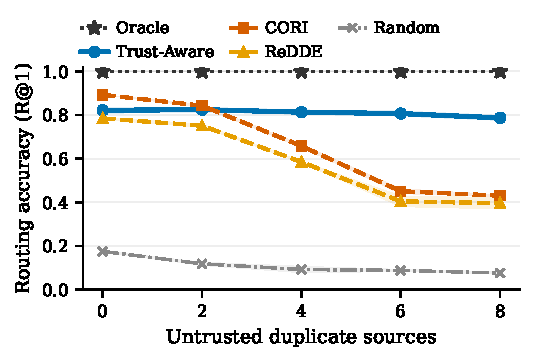
\includegraphics[width=0.92\columnwidth]{fig_robustness_routing.pdf}\\[2pt]
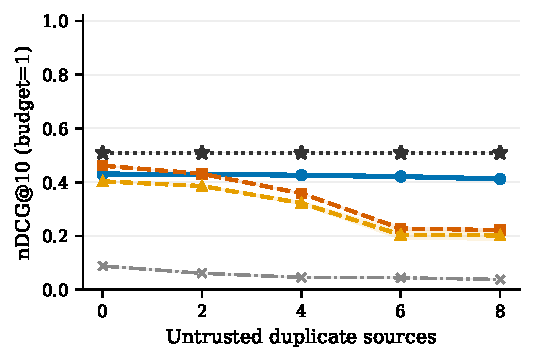
\includegraphics[width=0.92\columnwidth]{fig_robustness_ndcg.pdf}
\caption{Robustness to untrusted duplicate sources (mean$\pm$std, 3 seeds).
(top) routing accuracy $R@1$; (bottom) end-to-end nDCG@10 at budget $1$.
Content-based selection (CORI, ReDDE) collapses past two twins; \system{} stays
flat.}
\label{fig:robust}
\end{figure}

\begin{figure}[t]
\centering
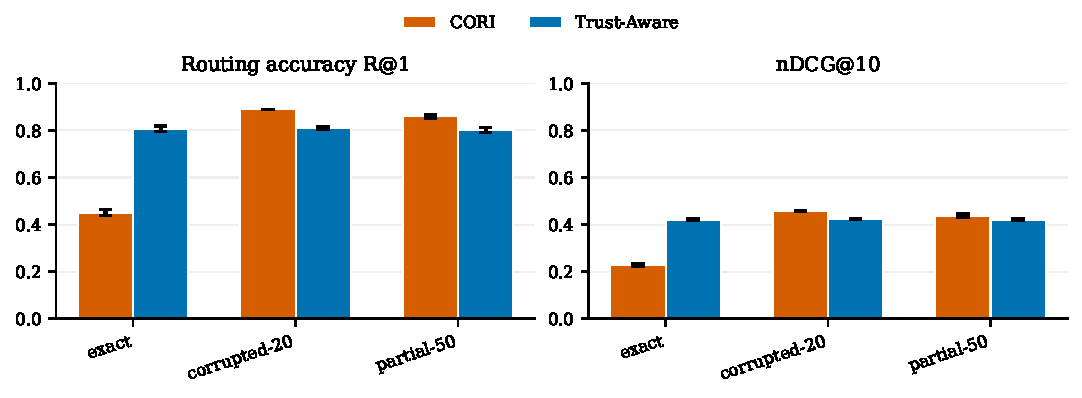
\includegraphics[width=0.95\columnwidth]{fig_adversary_variants.pdf}
\caption{Adversary-variant sensitivity at six untrusted sources. \system{} is
flat across exact, corrupted-20, and partial-50 mirrors; content-based routing
recovers only once the mirror's content statistics diverge from the genuine
source.}
\label{fig:variants}
\end{figure}

\subsection{RQ3: Are the gains statistically significant?}
Table~\ref{tab:sig} reports query-clustered paired tests at six twins over
$N_q=776$ independent queries. \system{} improves nDCG@10 over CORI by $+0.193$
(95\% CI $[0.173,0.214]$, $p_{\text{Holm}}=4.9\times10^{-59}$,
$r_{\mathrm{rb}}=0.809$) and over ReDDE by $+0.217$ (95\% CI $[0.196,0.238]$,
$p_{\text{Holm}}=2.6\times10^{-66}$, $r_{\mathrm{rb}}=0.841$). MAP shows the same
picture, with gains of $+0.170$ over CORI and $+0.190$ over ReDDE
($p_{\text{Holm}}\le 1.5\times10^{-66}$). All four comparisons have large paired
effects and reject the null after family-wise correction.

\begin{table}[t]
\centering
\caption{Significance of \system{} vs.\ baselines at six twins. Seed replicates
are averaged within query; tests are paired Wilcoxon with family-wise Holm
correction, query-bootstrap 95\% CIs, and rank-biserial effects.}
\label{tab:sig}
\scriptsize
\resizebox{\columnwidth}{!}{\begin{tabular}{llrrrrl}
\toprule
Metric & vs.\ & $N_q$ & $\Delta$ & 95\% CI & $p_{\text{Holm}}$ & $r_{\mathrm{rb}}$ (effect) \\
\midrule
nDCG@10 & CORI & 776 & +0.193 & [+0.173, +0.214] & 4.9e-59 & +0.809 (large) \\
nDCG@10 & ReDDE & 776 & +0.217 & [+0.196, +0.238] & 2.6e-66 & +0.841 (large) \\
MAP & CORI & 776 & +0.170 & [+0.152, +0.190] & 1.5e-66 & +0.825 (large) \\
MAP & ReDDE & 776 & +0.190 & [+0.170, +0.209] & 1.5e-74 & +0.854 (large) \\
\bottomrule
\end{tabular}
}
\end{table}

\subsection{RQ4: How important is the trust estimator?}
Table~\ref{tab:online} and Fig.~\ref{fig:online} compare \system{} with online
reputation ablations that receive the same feedback stream. CORI+Mean tests a
simple empirical-success multiplier, while CORI+UCB tests optimistic exploration.
All online trust variants recover most of the loss suffered by content-only
routing; on this testbed CORI+UCB is strongest on quality ($R@1=0.841$,
nDCG@10$=0.436$) and also marginally cheapest (cost $0.428$ vs.\ \system's $0.433$),
so \system{} is not dominant among feedback-driven methods---we report this rather
than hide it. The central effect is therefore first-class learned trust itself
rather than any particular posterior summary: once a source's observed outcomes
inform routing, all three variants recover, and the choice between an optimistic
upper bound and a conservative lower bound moves quality by less than $0.035$
$R@1$ and cost by about $0.005$. That the simple content-only CORI sits far below
all three ($R@1=0.451$) isolates the trust term, not the feedback plumbing, as the
source of the gains.

\begin{table}[t]
\centering
\caption{Online trust-estimator ablations at six twins (mean\,$\pm$\,std over
seeds, budget $b{=}1$). Bold marks the best value in each column.}
\label{tab:online}
\small
\begin{tabular}{l cccc}
\toprule
Method & R@1 & nDCG@10 & MAP & cost \\
\midrule
CORI & 0.451\,$\pm$\,0.011 & 0.228\,$\pm$\,0.006 & 0.187\,$\pm$\,0.007 & 0.441 \\
CORI+Mean & 0.832\,$\pm$\,0.011 & 0.430\,$\pm$\,0.001 & 0.362\,$\pm$\,0.002 & 0.429 \\
CORI+UCB & \textbf{0.841\,$\pm$\,0.009} & \textbf{0.436\,$\pm$\,0.003} & \textbf{0.365\,$\pm$\,0.003} & \textbf{0.428} \\
Trust-Aware & 0.807\,$\pm$\,0.012 & 0.421\,$\pm$\,0.003 & 0.357\,$\pm$\,0.001 & 0.433 \\
\bottomrule
\end{tabular}

\end{table}

\begin{figure}[t]
\centering
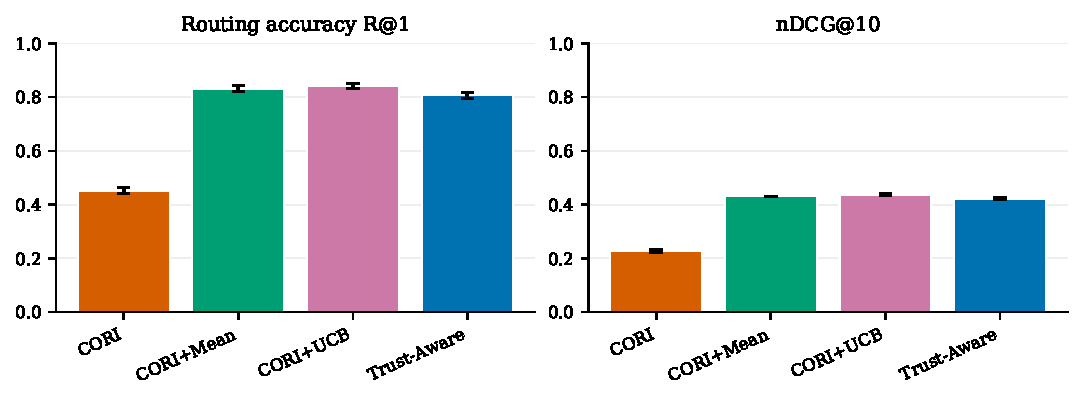
\includegraphics[width=0.95\columnwidth]{fig_online_baselines.pdf}
\caption{Online reputation ablations at six twins. Calibrated trust (any
posterior summary) recovers most of the content-only loss; the choice of summary
shifts quality and cost only marginally, with the optimistic CORI+UCB bound
slightly ahead of \system{} on both.}
\label{fig:online}
\end{figure}

\subsection{RQ5: How does the cost budget interact with trust?}
Table~\ref{tab:budget} reports end-to-end nDCG@10 at budgets $b\in\{1,2,3\}$ on
the six-twin federation. \system{} leads at every budget, but its most efficient
operating point is $b{=}1$: routing to the single most-trusted source yields
nDCG@10 $0.421$ at cost $0.433$---better than \emph{any} budget of either
baseline. Increasing the budget actually \emph{lowers} \system's nDCG@10
($0.421\!\rightarrow\!0.371\!\rightarrow\!0.336$), because querying additional
sources merges in twin and off-home results that dilute the top of the ranking---a
property of the merge, not of trust. The lesson is sharp: when trust is reliable,
spending budget to hedge across sources is counterproductive; the value of the
trust signal is precisely that it lets a router commit to one source confidently
and cheaply.

\begin{table}[t]
\centering
\caption{Budget interaction at six twins (end-to-end nDCG@10 and average cost,
mean over seeds). \system{} leads at every budget; its cheapest budget ($b{=}1$)
is also its best operating point.}
\label{tab:budget}
\small
\begin{tabular}{l cc cc cc}
\toprule
& \multicolumn{2}{c}{$b{=}1$} & \multicolumn{2}{c}{$b{=}2$} & \multicolumn{2}{c}{$b{=}3$}\\
\cmidrule(lr){2-3}\cmidrule(lr){4-5}\cmidrule(lr){6-7}
Method & nDCG@10 & cost & nDCG@10 & cost & nDCG@10 & cost \\
\midrule
ReDDE & 0.204 & 0.522 & 0.293 & 1.047 & 0.264 & 1.665 \\
CORI & 0.228 & 0.441 & 0.319 & 0.883 & 0.281 & 1.356 \\
\textbf{Trust-Aware} & 0.421 & 0.433 & 0.371 & 0.987 & 0.336 & 1.380 \\
\bottomrule
\end{tabular}

\end{table}

\subsection{RQ6: Does online calibration work, and what does it learn?}
Figure~\ref{fig:learn} (top) plots mean rolling routing accuracy over all three
query streams at six twins: \system{} stabilizes near $0.8$ within the first
window and holds it, while CORI and ReDDE remain much lower. The lower panel
shows final trust lower bounds for the representative seed-7 run. Frequently
sampled failing twins are demoted well below the optimistic prior; a rarely
selected twin remains near the prior, making explicit that the model changes
trust \emph{only} when it receives evidence---never by assumption.

\begin{figure}[t]
\centering
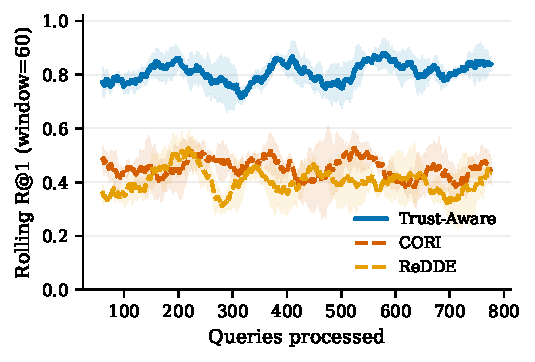
\includegraphics[width=0.99\columnwidth]{fig_learning_curve.pdf}\\[2pt]
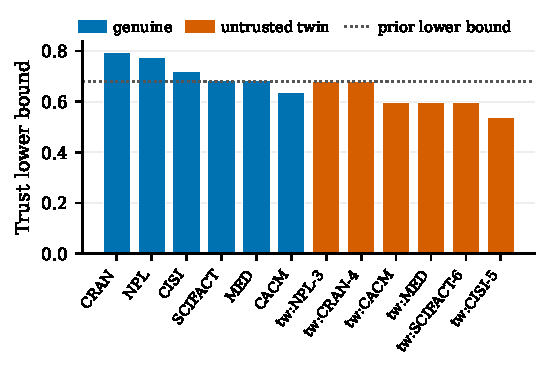
\includegraphics[width=0.92\columnwidth]{fig_learned_trust.pdf}
\caption{(top) Online calibration at six twins: mean rolling routing accuracy
with $\pm1$ standard-deviation bands across three seeds. (bottom) Final trust
lower bounds for seed 7; the dotted line is the optimistic-prior lower bound.}
\label{fig:learn}
\end{figure}

\subsection{RQ7: What does trust cost?}
Nothing, in budget terms. \system{} carries one beta--binomial pair per source
and an $O(n\log n)$ ranking per query; the trust update is $O(1)$. Its average
query cost at its $b{=}1$ operating point undercuts both content baselines
($0.433$ vs.\ $0.441$ for CORI and $0.522$ for ReDDE; Table~\ref{tab:budget}).
Two honest qualifications: at $b{=}2$ and $b{=}3$ \system{} is dearer than CORI
($0.987$ vs.\ $0.883$ and $1.380$ vs.\ $1.356$), though those budgets are worse
operating points for it anyway (RQ5); and the CORI+UCB reputation ablation is
marginally cheaper still at $b{=}1$ ($0.428$; Table~\ref{tab:online}). Fig.~\ref{fig:cleanvsdirty} contrasts clean vs.\ untrusted
operating points side by side: \system{} retains nearly all of its accuracy where
content-based selection sheds half of its own.

\begin{figure}[t]
\centering
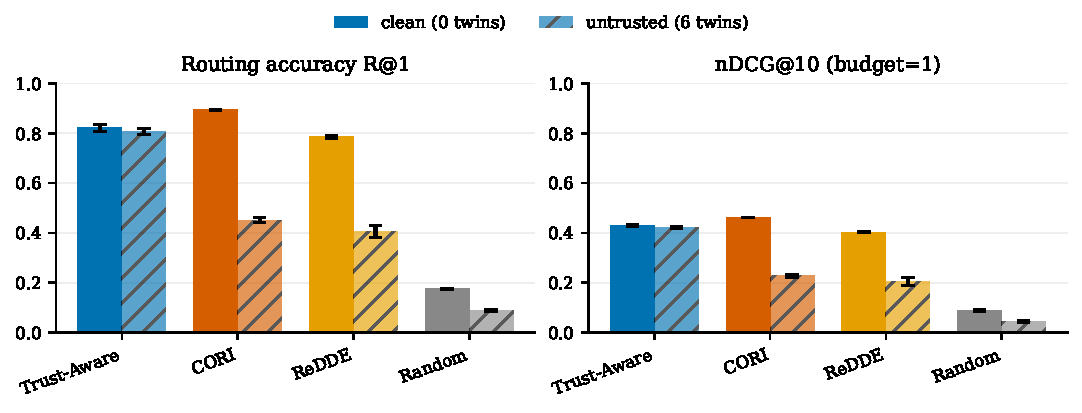
\includegraphics[width=0.99\columnwidth]{fig_clean_vs_untrusted.pdf}
\caption{Clean (0 twins) vs.\ untrusted (6 twins) federations. \system{} retains
most of its accuracy; content-based selection does not.}
\label{fig:cleanvsdirty}
\end{figure}

\section{Generalizing the Threat Model}\label{sec:extended}

The exact-twin model is deliberately the hardest content-blindness case, but a
skeptic may ask whether it is \emph{too} stylized: real impostors are rarely
either perfectly reliable or perfectly useless, and reliability is rarely fixed.
We therefore stress the trust layer along three further axes. All three reuse the
same six-collection testbed, CORI signal, and prequential protocol, and all
reproduce from \texttt{examples/run\_extended\_study.py}.

\subsection{RQ8: Graded/stochastic poisoning and calibration recovery}
We replace the all-or-nothing twin with a \emph{graded mirror} that returns a
genuine answer with probability $p\in\{0.0,0.2,0.4,0.6,0.8\}$---a faithful model
of a partially poisoned store or a stale replica that is right some of the time.
The question is not only whether \system{} routes well, but whether its posterior
\emph{recovers} the true reliability, which is what makes graceful degradation
possible.

It does. Table~\ref{tab:calibration} shows that the learned posterior mean tracks
the injected reliability closely across the whole range: the mirror mean-absolute
error between true $p$ and learned $\hat\mu$ is $0.068$ with Pearson correlation
$r=0.988$, and genuine sources are correctly learned to be highly reliable
($\hat\mu\approx 0.95$). Figure~\ref{fig:calibration} plots learned trust against
true reliability and shows the points lying close to the diagonal, with the lower
confidence bound sitting just below the mean as the conservative summary used for
routing. This directly rebuts the ``evil twins are too stylized'' objection: the
mechanism is not a twin detector, it is a reliability estimator, and it works for
the entire continuum between genuine and useless.

\begin{table}[t]
\centering
\caption{Graded-poisoning calibration (RQ8). Mirrors return genuine answers with
probability \emph{True $p$}; the learned posterior mean $\hat\mu$ and lower bound
$\tau$ recover it (mirror MAE $0.068$, Pearson $r=0.988$). Means over seeds
$\{7,11,13\}$.}
\label{tab:calibration}
\small
\begin{tabular}{l ccccc}
\toprule
Injected source & True $p$ & Realised & Learned $\hat\mu$ & Learned LCB $\tau$ & \#obs \\
\midrule
mirror & 0.00 & 0.000 & 0.129\,$\pm$\,0.000 & 0.087 & 52 \\
mirror & 0.20 & 0.222 & 0.367\,$\pm$\,0.066 & 0.292 & 30 \\
mirror & 0.40 & 0.376 & 0.417\,$\pm$\,0.024 & 0.369 & 93 \\
mirror & 0.60 & 0.616 & 0.624\,$\pm$\,0.036 & 0.593 & 225 \\
mirror & 0.80 & 0.798 & 0.798\,$\pm$\,0.029 & 0.756 & 76 \\
\midrule
genuine (mean of 6) & 0.970 & -- & 0.948 & -- & -- \\
\bottomrule
\end{tabular}

\end{table}

\begin{figure}[t]
\centering
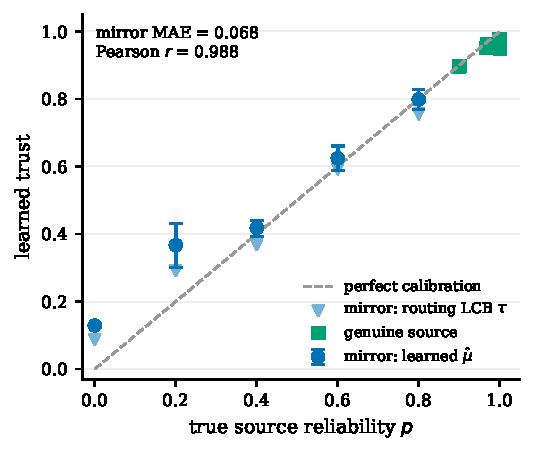
\includegraphics[width=0.95\columnwidth]{fig_calibration.pdf}
\caption{Calibration under graded poisoning (RQ8): learned trust vs.\ true
reliability. Points lie close to the diagonal across the full $[0,1]$ range;
the lower bound (routing summary) sits just below the posterior mean.}
\label{fig:calibration}
\end{figure}

\subsection{RQ9: Non-stationary reliability (drift)}
Reliability is not static: a stale mirror may be refreshed, or a fresh source may
be poisoned. We construct two content-identical mirrors whose reliability
\emph{changes mid-stream}---one stale-then-refreshed, one fresh-then-poisoned---
with the regime change at the halfway point of the target's query stream.
Figure~\ref{fig:drift} plots the trust trajectories. The online estimator
re-calibrates after the change so that the two trajectories \emph{cross}: the
source that becomes reliable rises and the one that becomes poisoned falls. No
static content signal can produce this behavior, because both mirrors are
lexically identical to their genuine source throughout; only an outcome-driven
estimator can follow a moving target. This is the property that makes \system{}
suitable for the open, drifting federations of Section~\ref{sec:related}: trust
is continually re-earned, never assumed.

\begin{figure}[t]
\centering
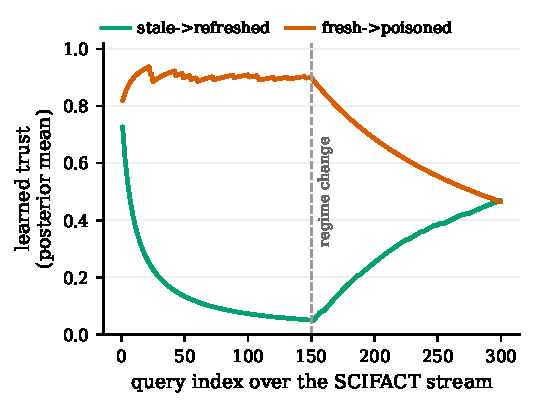
\includegraphics[width=0.95\columnwidth]{fig_drift.pdf}
\caption{Non-stationary reliability (RQ9). Two content-identical mirrors whose
reliability changes at mid-stream (vertical line). The online trust trajectories
re-calibrate and cross---behavior no static content signal can exhibit.}
\label{fig:drift}
\end{figure}

\subsection{RQ10: Hyper-parameter sensitivity}
Finally we map the method's robustness to its two free knobs: the optimistic prior
$(\alpha_0,\beta_0)$ and the lower-bound width $z$. Table~\ref{tab:hyperparam}
reports end-to-end nDCG@10 over a $4\times 3$ grid at six twins. Across every
optimistic prior---all nine cells with $(\alpha_0,\beta_0)\in\{(4,2),(8,2),(20,5)\}$,
which is the regime the method is specified for---it is stable (nDCG@10
$\in[0.376,0.434]$), and the default $(8,2),z{=}1$ sits comfortably inside that
band. Degradation is confined to the \emph{flat} prior $(1,1)$, and there it is
graded in $z$: $0.404$ at $z{=}0$, $0.331$ at $z{=}1$, and a collapse to $0.025$ at
$z{=}2$, which we report rather than hide, because a flat prior
gives a fresh source high posterior variance and a wide lower bound then drives
its trust to zero before any evidence arrives---freezing the router. The failure
is interpretable and points directly to the design choice: an \emph{optimistic}
prior is what lets a never-yet-observed reliable source be tried at all. With any
non-degenerate prior the method is insensitive to $z$, confirming that the
defaults are a safe, principled operating point rather than a tuned sweet spot.

\begin{table}[t]
\centering
\caption{Hyper-parameter sensitivity at six twins (RQ10): end-to-end nDCG@10 over
a $4\times3$ grid of prior $(\alpha_0,\beta_0)$ and lower-bound width $z$. Robust
across the sensible region; the one degenerate corner (flat prior, aggressive
$z$) motivates the optimistic default. Bold marks the default.}
\label{tab:hyperparam}
\small
\begin{tabular}{l ccc}
\toprule
Prior $(\alpha_0,\beta_0)$ & $z=0$ & $z=1$ & $z=2$ \\
\midrule
$(1,1)$ & 0.404 & 0.331 & 0.025 \\
$(4,2)$ & 0.421 & 0.402 & 0.376 \\
$(8,2)$ & 0.430 & \textbf{0.421} & 0.406 \\
$(20,5)$ & 0.434 & 0.432 & 0.425 \\
\bottomrule
\end{tabular}

\end{table}

\section{Discussion and Limitations}\label{sec:discussion}

We report limitations candidly. (i)~The collections are real and standard but
modest in scale; the design is dataset-agnostic and ports directly to large
modern federations (e.g., BEIR shards~\cite{thakur2021beir}), which is the most
important next step for external validity. (ii)~We study single-home routing;
multi-home queries, where evidence is spread across sources, are a natural
extension and would interact with the budget effect in RQ5. (iii)~Retrieval is
lexical (BM25); the trust mechanism is orthogonal to the base retriever and should
compose with neural rankers, since it multiplies whatever relevance score is
supplied. (iv)~The evil-twin model treats unverifiable duplicates as non-relevant
under the standard pooling assumption; the graded, drift, and degraded-mirror
studies (Sections~\ref{sec:results},~\ref{sec:extended}) show the boundary---when
content statistics change, content-based routers can recover, while
content-equivalent contamination remains the hard case. (v)~The online feedback
signal is a proxy for real user or verification feedback; in deployment this
outcome would come from downstream answer validation, click signals, or an
auditing layer.

\subsection{Threats to validity}
\emph{Construct validity.} Our outcome label---``did the routed source return a
judged-relevant document?''---is a reasonable but imperfect proxy for
trustworthiness; a source could return relevant-looking but subtly wrong content.
The graded-poisoning study (RQ8) partly addresses this by decoupling reliability
from content. \emph{Internal validity.} The prequential protocol eliminates
train/test leakage, and identical seeded tie-breaking is applied to every method,
so \system{} is granted no structural advantage. \emph{External validity.} Six
collections in six domains, spanning both classic corpora and a modern BEIR
collection, is a genuine federation but not web-scale; the contamination sweep,
retention metric, and reproduction harness are designed to transfer unchanged to
larger testbeds. Absolute metric values are also sensitive to judgment density:
SciFact's $\approx1.1$ relevant documents per query lift every method's nDCG@10,
Oracle included, so absolute values should not be compared across testbed
revisions---only differences between methods on a fixed testbed. \emph{Statistical-conclusion validity.}
We treat the 776 queries as the independent units, average seed replicates within
query, and apply family-wise Holm correction across the full comparison family,
so the reported significance is conservative.

\subsection{Ethical considerations and responsible deployment}
A trust estimator that demotes sources is a governance mechanism, and like any
such mechanism it can be misused. Two cautions are worth stating. First, trust
here is \emph{behavioral and per-source}, learned from outcomes; it is not a
judgment about content quality, authorship, or any protected attribute, and it
should not be repurposed as one. Second, an outcome-driven estimator can in
principle be gamed by an adversary who supplies genuinely useful answers until
trusted and then defects; the drift study (RQ9) shows the estimator re-demotes
such a source once it starts failing, but the lag depends on query volume, so
safety-critical deployments should pair the routing-layer signal with
document-level verification~\cite{zhong2023corpus,zou2025poisonedrag} rather than
relying on either alone. We see provenance-robust routing as one layer of
defense-in-depth, not a complete solution. None of these caveats undermine the
core finding: content-based selection is provenance-blind, loses roughly half its
quality to impostors it cannot see, and a calibrated, learned trust objective
closes the gap at no additional cost.

\section{Conclusion}\label{sec:conclusion}

We made the case that trust must be a first-class routing objective in AI-native
data systems, and showed why: content-based resource selection cannot see
provenance and collapses when untrusted duplicate sources enter the federation---
a failure we prove is fundamental, not incidental (Proposition~\ref{prop:bound}).
\system{} combines a content-relevance signal with an online-calibrated
beta--binomial trust estimate and routes by expected utility under a budget. On a
fully reproducible federation of six real collections it is competitive on clean
data and dramatically more robust to untrusted sources---retaining $96\%$ of its
clean accuracy under heavy contamination where content baselines retain roughly
half---with large, highly significant gains at a cost below both content
baselines at its single-source operating point. Beyond exact twins, the learned posterior recovers graded reliability,
tracks non-stationary drift, and is robust across its hyper-parameters. We hope
the testbed, the contamination sweep, the retention metric, and the generalized
threat model make provenance-robust routing a standard axis of evaluation for
AI-native data systems.

\section*{CRediT authorship contribution statement}
Jorge Martinez-Gil: Conceptualization, Methodology, Software, Validation, Formal
analysis, Investigation, Data curation, Visualization, Writing - original draft,
Writing - review and editing.

\section*{Declaration of competing interest}
The author declares that he has no known competing financial interests or
personal relationships that could have appeared to influence the work reported in
this paper.

\section*{Funding}
This research did not receive any specific grant from funding agencies in the
public, commercial, or not-for-profit sectors.

\section*{Data and code availability}
All datasets, baselines, statistics, figures, and tables in this paper regenerate
from the released artifact at
\url{https://github.com/jorge-martinez-gil/trust-aware}. The core study reruns
with \texttt{python -m trust\_aware -{}-federated-study} and the generalized
threat-model study (Section~\ref{sec:extended}) with
\texttt{examples/run\_extended\_study.py}. A regression test asserts the headline
robustness claim, and an internal consistency check cross-validates the headline
constants against the cached result JSON, so every number above is traceable to a
fresh run. The bundled IR collections are documented with provenance metadata
and per-collection licence terms in the artifact: the five classic collections are
public domain, while SciFact's claims are CC BY 4.0 over S2ORC abstracts under
ODC-By 1.0.

\section*{Declaration of generative AI and AI-assisted technologies in the
manuscript preparation process}
During the preparation of this work the author used OpenAI Codex to assist with
language editing, LaTeX formatting, and submission-compliance checks. After using
this tool, the author reviewed and edited the content as needed and takes full
responsibility for the content of the published article.

\section*{Acknowledgments}
We thank the maintainers of the public CACM, MED, NPL, CRAN, and CISI
collections, and the authors of SciFact~\cite{wadden2020fact} and of the BEIR
benchmark~\cite{thakur2021beir}, whose openly available data made a fully
reproducible federated testbed possible.

\bibliographystyle{elsarticle-num}
\bibliography{references}

\end{document}
